\documentclass[11 pt, letterpaper]{report}


\usepackage[utf8]{inputenc}
\usepackage
{
 authblk,
 xcolor,
 listings,
 hyperref,
 graphicx,
 tcolorbox
}


\newcommand{\R}{\textcolor{red}}
\newcommand{\T}{\texttt}
\renewcommand\contentsname{Aidike Taka}


\title{Python}
\author
{
 Sofiullah Iqbal Kiron\\
 Mail: \href{mailto:sofiul.k.1023@gmail.com}{sofiul.k.1023@gmail.com}
}
\affil{BSMRSTU, Department of CSE}


\lstset
{
 language=python,
 backgroundcolor=\color{black!1},
 keywordstyle=\color{blue},
 stringstyle=\color{red},
 basicstyle=\tiny,
 numbers=left
}


\begin{document}

\maketitle
\tableofcontents

\section*{Introduction}
Reference: \href{https://www.youtube.com/watch?v=WGJJIrtnfpk&t=12362s}{edureka!}\\
HI, it is a great time to learn python programming. Before we began, let's talk about our agenda for today. We will give you a guided way of becoming a python developer.\\
\begin{enumerate}
 \item Comments
 \item Variable
 \item Operators
 \item Data types
 \item Loop
 \item Libraries
 \item File Handling and Functions
 \item Web developing and Web Scraping
\end{enumerate}

\subsection*{Introduction by Mosh}
Python is an interpreted language. An interpreter basically a program that converts the Human code to machine code. Python is implemented by C. We download default implementation of python from \href{python official website}{python.org}. Default implementation of python is called CPython. We can use Java codes in python through Jython.

\section*{Comment}
Python comment is oneline comment mode and this is written adding a before hash tag. \\
e.g. : \#This is a python comment.

\section*{Variable}
Let's continue this series on \textcolor{green}{PYTHON}. \\
Variables are a special container that stores value. In python, "Variable is Variable". So no need to specify primary stage declaration of type of a variable. That's why, Python called, dynamically typed programming language.
\subsection*{Value Assignment}
Syntax: \textcolor{red}{$variable\_name = value$} \\
Equal sign $( = )$ is used to assign values to the variable.
\subsection*{Value changing}
First we assign $2$ to the variable $x$ and then assign $9$ to the $x$. So, present value of $x$ is $9$.
$
x = 2\\
x  9\\
$
Now, $x=9$.
\\
If we want to access output of previous operation, use underscore $( _ )$. This means output of previous operation.
\\e.g. : $10 + x\\
= 19\\
y = 2\\
\_+ y\\
= 21\\
$
\subsection*{String Variable}
String concatenation in Python is same as C++. Use $+$ sign to concatenate.\\
Declaring string variable:\\
Syntax: \textcolor{red}{variable\_name='Name'}\\
e.g. : platform = 'YouTube'\\
IN: platform[0]\\
OP: 'Y'\\
Normally in computer, counting always starts with 0.\\
IN: platform[1:4]\\
OP: ouT\\
That means, first one is starting index, second-one is before ending index.\\
Let's use len() function for outcome the length of the string variable.\\
IN: len(platform)\\
OP: 7\\
It returns an integer, size of platform.\\
\begin{flushright}
\textbf{Fourth tutorial over.}
\end{flushright}

\section*{Loop}
\subsection*{For Loop}
Now we will talk about \textcolor{red}{for} loop.\\
We can write \textcolor{red}{if} inside a \textcolor{red}{for}. If we have \textcolor{red}{if} inside a \textcolor{red}{for}, then we have \textcolor{red}{for} inside a \textcolor{red}{for}.\\
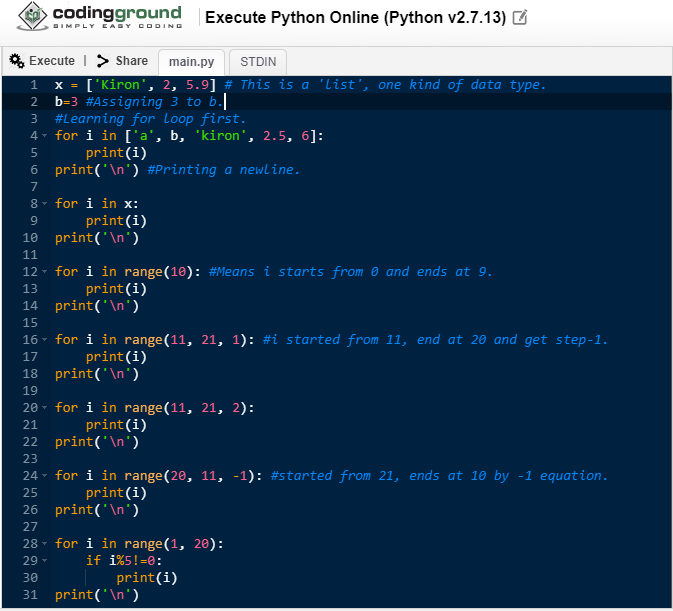
\includegraphics[width=260 px, height=230 px]{For Loop practice.png}

List is a great kind of data type in Python. Here 'x' is a list variable. We will discuss about it later.

\section*{Functions}
In python, user-defined functions are starts with \textcolor{red}{"def"} keyword.
\begin{lstlisting}
def fun_name():
	print("Kiron")
	
fun_name() #Calling the function.
\end{lstlisting}
\begin{tcolorbox}
Output: Kiron
\end{tcolorbox}

\subsection*{Multiple return value}
This is how we return multiple values from a python \textcolor{red}{"def"}\\
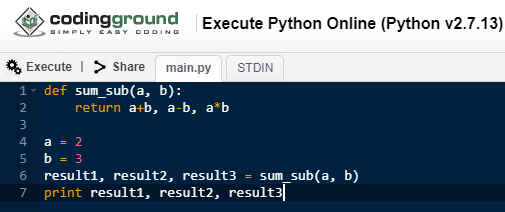
\includegraphics[width=200 px]{Multiple return value from function def.png}
\begin{tcolorbox}
Output: 5, -1, 6
\end{tcolorbox}

\pagebreak

\section*{PIP}
PIP: Python Installer Package \\
\begin{enumerate}
	\item[Check version:] \R{\T{pip --version}}
	\item [List installed packages:] \R{\T{pip list}}
	\item[Update:] browse the directory where python is installed then run the command, \R{\T{python -m pip install --upgrade pip}}
	\item [Install a package:] \R{\T{pip install package\_name}}
	\item [Uninstall a package:] \R{\T{pip uninstall package\_name}}
	\item[Show:] information about a package briefly, \R{\T{py -m pip show package\_name}}
	\item[Show:] information about a package descriptively, \R{\T{py -m pip show --verbose package\_name}}
\end{enumerate}
Documentation \href{https://pip.pypa.io/en/stable/}{\textcolor{blue}{here}}.

\end{document}